\documentclass[12pt,letterpaper]{article}
\usepackage{fullpage}
\usepackage[top=2cm, bottom=4.5cm, left=2.5cm, right=2.5cm]{geometry}
\usepackage{amsmath,amsthm,amsfonts,amssymb,amscd}
\usepackage{lastpage}
\usepackage{enumerate}
\usepackage{fancyhdr}
\usepackage{mathrsfs}
\usepackage{xcolor}
\usepackage{graphicx}
\usepackage{listings}
\usepackage{hyperref}
\usepackage{tikz}
\usepackage{xfrac}
\usepackage{nicefrac}
\usepackage{xcolor}

\usetikzlibrary{shapes.geometric,fit}

\hypersetup{
  colorlinks=true,
  linkcolor=blue,
  linkbordercolor={0 0 1}
}

\setlength{\parindent}{0.0in}
\setlength{\parskip}{0.05in}


\newcommand\course{ECON 3211}
\newcommand\hwnumber{2}
\newcommand\NetIDa{dc3451}
\newcommand\NetIDb{David Chen}          

\theoremstyle{definition}
\newtheorem*{statement}{Statement}
\newtheorem*{claim}{Claim}
\newtheorem*{theorem}{Theorem}

\newcommand{\contra}{\Rightarrow\!\Leftarrow}

\pagestyle{fancyplain}
\headheight 35pt
\lhead{\NetIDa}
\lhead{\NetIDa\\\NetIDb}
\chead{\textbf{\Large Problem Set \hwnumber}}
\rhead{\course \\ \today}
\lfoot{}
\cfoot{}
\rfoot{\small\thepage}
\headsep 1.5em

\begin{document}

\section*{Math Review}
\subsection*{a)}

\begin{alignat*}{2}
    && dU = \frac{\delta U}{\delta x}dx + \frac{\delta U}{\delta y}dy &= 0 \\
    &\implies& -\frac{\delta U}{\delta y}dy &= \frac{\delta U}{\delta x}dx \\
    &\implies& \frac{dy}{dx} &= -\frac{\frac{\delta U}{\delta x}}{\frac{\delta U}{\delta y}}
\end{alignat*}

\subsection*{b)}

\begin{alignat*}{2}
    && R(x,y) &= \$10x + \$5y - \$100 = 0 \\
    &\implies& dR &= \frac{\delta R}{\delta x}dx + \frac{\delta R}{\delta y}dy = \$10dx + \$5dy = 0 \\
    &\implies& \frac{dy}{dx} &= -2
\end{alignat*}

\subsection*{c)}

This does not exist for some reason.

\subsection*{d)}
\begin{align*}
    \mathcal{L}(x, y, \lambda) &= 2x^{0.5} + 2y^{0.5} -\lambda(x + y - 16) 
\end{align*}

\subsection*{e)}
\begin{align*}
    \mathcal{L}(x, y, \lambda) &= x + y - \lambda(x^2 + y^2 - 16) 
\end{align*}

\section*{Problem 1}
(What a terrible world to live in.)

\subsection*{a)}
\subsubsection*{a.1, \textcolor{red}{a.2}}
\begin{center}
    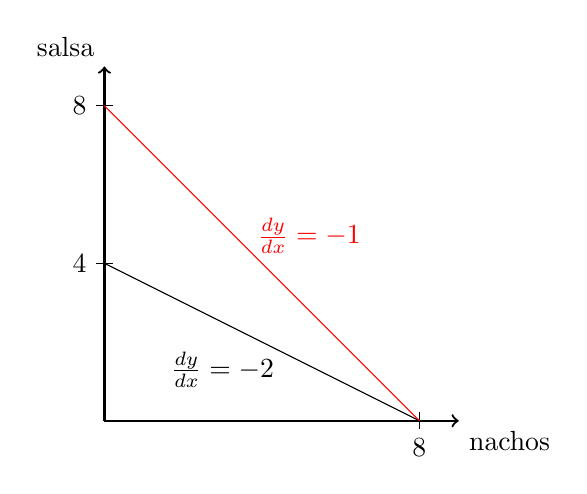
\begin{tikzpicture}
        \draw[thick,->] (0,0) -- (4.5,0) node[anchor=north west] {nachos};
        \draw[thick,->] (0,0) -- (0,4.5) node[anchor=south east] {salsa};
        \draw (4cm,3pt) -- (4cm,-3pt) node[anchor=north] {$8$}; 
        \draw (3pt,2cm) -- (-3pt,2cm) node[anchor=east] {$4$};
        \draw (4cm,0) --  node[below,xshift=-5mm] {$\frac{dy}{dx} = -2$} (0, 2cm);
        
        \draw (3pt,4cm) -- (-3pt,4cm) node[anchor=east] {$8$};        
        \draw[red] (4cm,0) --  node[above,xshift=6mm] {$\frac{dy}{dx} = -1$} (0, 4cm);
    \end{tikzpicture}
\end{center}

\subsubsection*{a.3, \textcolor{red}{a.4}}
Note that this is the same exact situation as above before the price shift. $S$ is the inital bundle of goods.
\begin{center}
    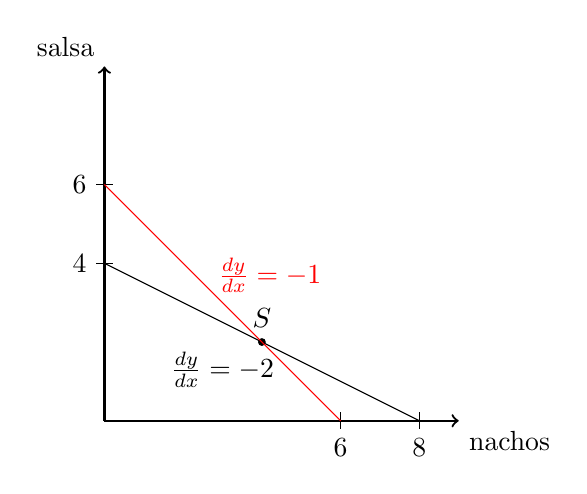
\begin{tikzpicture}
        \draw[thick,->] (0,0) -- (4.5,0) node[anchor=north west] {nachos};
        \draw[thick,->] (0,0) -- (0,4.5) node[anchor=south east] {salsa};
        \draw (4cm,3pt) -- (4cm,-3pt) node[anchor=north] {$8$}; 
        \draw (3pt,2cm) -- (-3pt,2cm) node[anchor=east] {$4$};
        \draw (4cm,0) --  node[below,xshift=-5mm] {$\frac{dy}{dx} = -2$} (0, 2cm);
        \draw (2cm,1cm) node[circle,fill,inner sep=1pt,label=above:$S$]{};
        
        \draw (3pt,3cm) -- (-3pt,3cm) node[anchor=east] {$6$};        
        \draw (3cm,3pt) -- (3cm,-3pt) node[anchor=north] {$6$};        

        \draw[red] (3cm,0) --  node[above,xshift=6mm] {$\frac{dy}{dx} = -1$} (0, 3cm);
    \end{tikzpicture}
\end{center}

\subsection*{b)}
\subsubsection*{b.1}
\begin{center}
    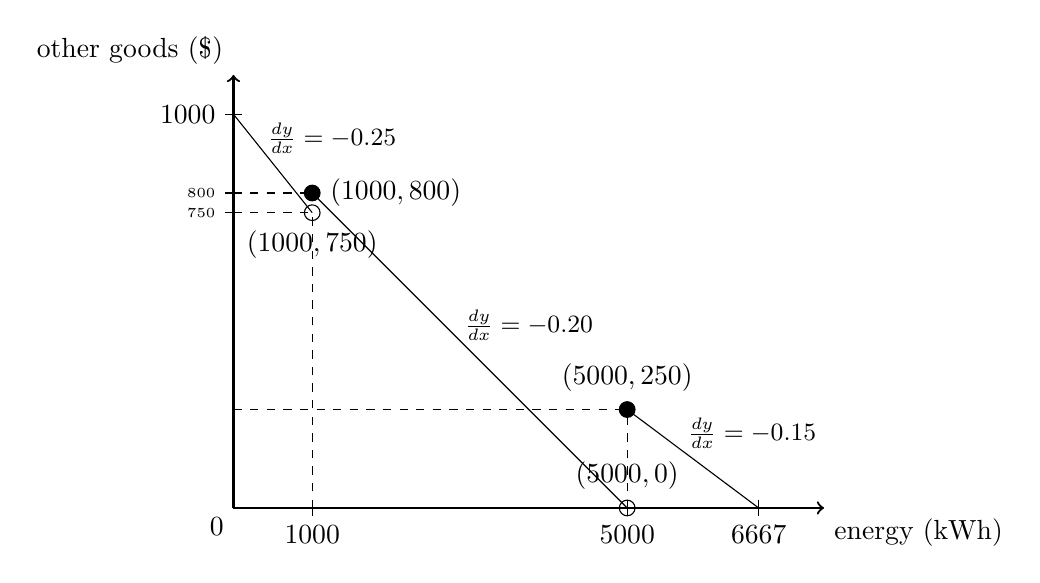
\begin{tikzpicture}[
            dot/.style={shape=circle, inner sep=2pt, draw, node contents=},
            circ/.style={shape=circle, inner sep=2pt, draw, fill}]
        \draw[thick,->] (0,0) -- (7.5,0) node[anchor=north west] {energy (kWh)};
        \draw[thick,->] (0,0) -- (0,5.5) node[anchor=south east] {other goods (\$)};
        \draw (6.67cm,3pt) -- (6.67cm,-3pt) node[anchor=north] {$6667$}; 
        \draw (1cm,3pt) -- (1cm,-3pt) node[anchor=north] {$1000$}; 
        \draw (5cm,3pt) -- (5cm,-3pt) node[anchor=north] {$5000$}; 

        \draw (3pt,5cm) -- (-3pt,5cm) node[anchor=east] {$1000$};
        \draw (3pt,4cm) -- (-3pt,4cm) node[anchor=east] {\tiny $800$};
        \draw (3pt,3.75cm) -- (-3pt,3.75cm) node[anchor=east] {\tiny $750$};
        
        \draw node[anchor=north east] {$0$};

        \draw (1cm,3.75cm) node[dot,label=below:{$(1000,750)$}]{};
        \draw (1cm,4cm) node[circ,label=right:{$(1000,800)$}]{};
        \draw (5cm,0cm) node[dot,label=above:{$(5000,0)$}]{};
        \draw (5cm,1.25cm) node[circ,label=above:{$(5000,250)$}]{};
        
        \draw (0,5cm) -- node[above,xshift=7.5mm,] {\small $\frac{dy}{dx} = -0.25$} (1cm,3.75cm);
        \draw (1cm,4cm) -- node[above,xshift=7.5mm] {\small $\frac{dy}{dx} = -0.20$}(5cm, 0cm);
        \draw (5cm,1.25cm) -- node[above,xshift=7.5mm] {\small $\frac{dy}{dx} = -0.15$} (6.67, 0cm);
        
        \draw[dashed] (1cm,0cm) -- (1cm,3.75cm);
        \draw[dashed] (5cm,0cm) -- (5cm,1.25cm);
        \draw[dashed] (0cm,3.75cm) -- (1cm,3.75cm);
        \draw[dashed] (0cm,4cm) -- (1cm,4cm);
        \draw[dashed] (0cm,1.25cm) -- (5cm,1.25cm);
    \end{tikzpicture}
\end{center}

\subsubsection*{b.2}
\begin{center}
    \[
    y = \begin{cases}
        1000 - 0.25x & 0 \leq x < 1000 \\
        1000 - 0.20x & 1000 \leq x < 5000 \\
        1000 - 0.15x & 5000 \leq x 
    \end{cases}
    \]
    
\end{center}

\subsection*{c)}
\subsubsection*{c.1}
\begin{center}
    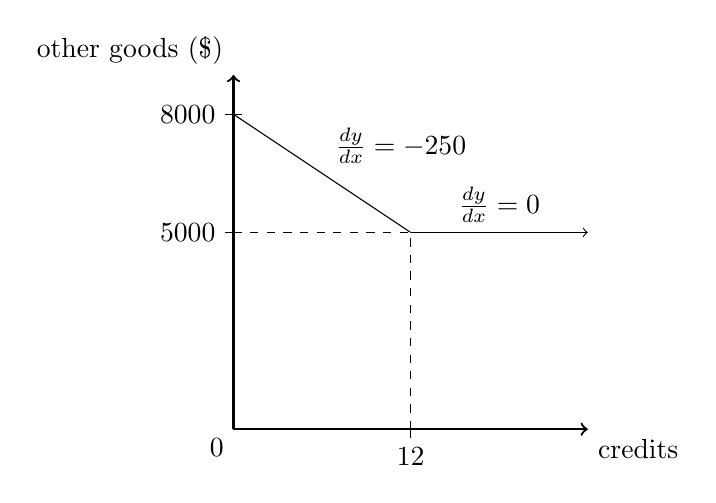
\begin{tikzpicture}[
            dot/.style={shape=circle, inner sep=2pt, draw, node contents=},
            circ/.style={shape=circle, inner sep=2pt, draw, fill}]
        \draw[thick,->] (0,0) -- (4.5,0) node[anchor=north west] {credits};
        \draw[thick,->] (0,0) -- (0,4.5) node[anchor=south east] {other goods (\$)};
        
        \draw (3pt,4cm) -- (-3pt,4cm) node[anchor=east] {$8000$};
        \draw (3pt,2.5cm) -- (-3pt,2.5cm) node[anchor=east] {$5000$};
        
        \draw (2.25cm,3pt) -- (2.25cm,-3pt) node[anchor=north] {$12$};
        
        \draw (0cm,4cm) -- node[above,xshift=10mm] {$\frac{dy}{dx} = -250$} (2.25cm,2.5cm);
        \draw[->] (2.25cm,2.5cm) -- node[above,] {$\frac{dy}{dx} = 0$} (4.5cm,2.5cm);
        
        \draw[dashed] (0cm, 2.5cm) -- (2.25cm, 2.5cm);
        \draw[dashed] (2.25cm, 0cm) -- (2.25cm, 2.5cm);

        \draw node[anchor=north east] {$0$};
    \end{tikzpicture}
\end{center}

\subsubsection*{c.2}
At 10 credits, the student has an opportunity cost of $\$250$ that could be spent on other goods for taking an extra credit.

However, at 13 credits, the student would just be paying the bulk payment of $\$3000$ for the semester, so there is no opportunity cost for another credit other than the time that she must invest into the credit.

\section*{Problem 2}
\subsection*{a)}
\subsubsection*{a.1}
\begin{center}
    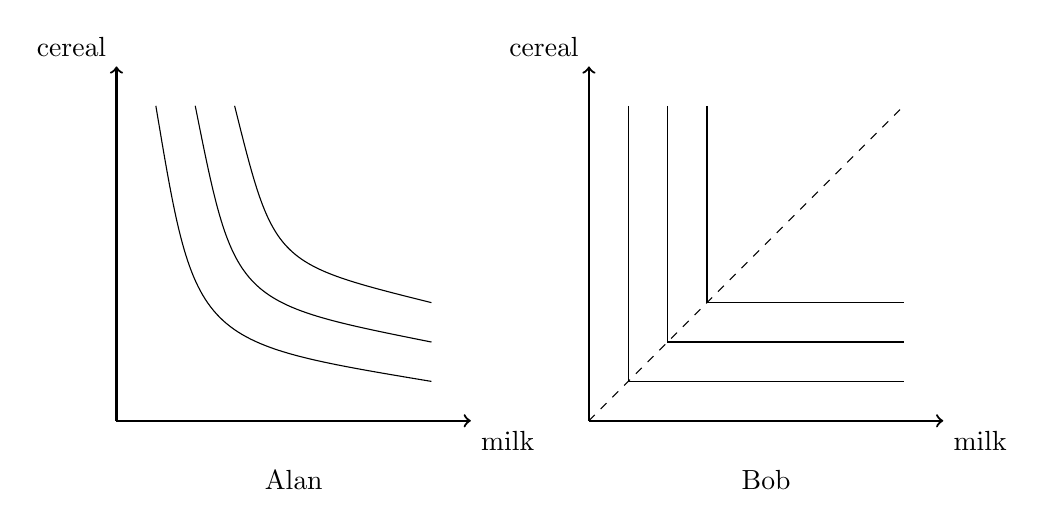
\begin{tikzpicture}[
            dot/.style={shape=circle, inner sep=2pt, draw, node contents=},
            circ/.style={shape=circle, inner sep=2pt, draw, fill}]
        \draw[thick,->] (0,0) -- node[below, yshift=-0.5cm] {Alan} (4.5,0) node[anchor=north west] {milk};
        \draw[thick,->] (0,0) -- (0,4.5) node[anchor=south east] {cereal};
        
        \draw (0.5,4) .. controls (1,1) .. (4,0.5);
        \draw (1,4) .. controls (1.5,1.5) .. (4,1);
        \draw (1.5,4) .. controls (2,2) .. (4,1.5);

        \draw[thick,->] (6,0) -- node[below, yshift=-0.5cm] {Bob} (10.5,0) node[anchor=north west] {milk};
        \draw[thick,->] (6,0) -- (6,4.5) node[anchor=south east] {cereal};
        
        \draw (6.5,4) -- (6.5,0.5) -- (10,0.5);
        \draw (7,4) -- (7,1) -- (10,1);
        \draw (7.5,4) -- (7.5,1.5) -- (10,1.5);
        
        \draw[dashed] (6,0) -- (10,4);  
		\end{tikzpicture}
\end{center}

\subsubsection*{a.2}
An example utility function for Alan can be the Cobbs-Douglas utility function, $U(q_c, q_m) = q_c^{0.5}q_m^{0.5}$.

An example utility function for Bob can be $U(q_c,q_m) = \min(q_c,q_m)$. The dashed line marks the kinks of the contours of the utility function.

\subsection*{b)}
\subsubsection*{b.1}

We have that $MRS_{Y,X} = -\frac{MU_X}{MU_Y}$.

\begin{align*}
		MU_X &= \frac{\delta U}{\delta x} = (y + z) \\
		MU_Y &= \frac{\delta U}{\delta y} = x \\
		\implies MRS_{Y,X} &= -\frac{y+z}{x}
\end{align*}

\subsubsection*{b.2}

$|MRS_{Y,X}|$ would fall from $\frac{y+100}{x}$ to $\frac{y+80}{x}$, a fall in magnitude of $\frac{20}{x}$.
This means that consumers would be less willing to substitute air travel for other goods (specifically they would be willing to give up $\frac{20}{x}$ less for an extra mile traveled by air).

\subsubsection*{b.3}

This makes sense, because after 9/11 airline safety would go down, so that consumers are less willing to sacrifice other spending for air travel, decreasing the amount of people traveling by air.
In the context of 9/11, this would suggest not particularly that people's tastes have changed, but their information has changed (9/11 makes consumers think that airline travel is unsafe), leading them to stay away from air travel.

\subsubsection*{b.4}

We now have that $MRS_{Y,X} = \frac{yz}{xz} = \frac{y}{x}$. This means that $MRS_{Y,Z}$ is independent of $Z$, which doesn't make that much sense, as you would expect a change in airline safety to either increase or decrease travel. 

In another sense this is strange also because $MU_Y = xz$. Why would the marginal utility of other spending depend specifically on the safety of air travel?

\section*{Problem 3}
\subsection*{a)}

Carla generally likes more even bundles (though skewed torwards clothes), as they appear to be imperfect substitutes to each other as shown by a Cobbs-Douglas utility function. However, since the exponent of clothing is higher in her utility function, we can conclude that she enjoys clothes more than food per each respective unit.

\subsection*{b)}

\begin{center}
		$MU_X = \frac{\delta U}{\delta x} = \frac{1}{3}x^{-2/3}y^{2/3} = \frac{1}{3}(\frac{y}{x})^{2/3}$.
\end{center}


This diminishes monotonically as $x$ increases, meaning that her marginal utility for food decreases as she consumes more food.

\subsection*{c)}

\begin{center}
		$5x + 25y = 900$ 
\end{center}

\subsection*{d)}

We can formally describe Carla's utility maximization problem as the following: find the maximum value of $U(x,y) = x^{1/3}y^{2/3}$ with $x,y \geq 0$ such that $5x + 25y = 900$.

\subsection*{e)}
\subsubsection*{e.1}
\begin{center}
		$\mathcal{L}(x,y,\lambda) = x^{1/3}y^{2/3} - \lambda(5x + 25y - 900)$
\end{center}

\subsubsection*{e.2}
\begin{align*}
		\frac{\delta \mathcal{L}}{\delta x} &= \frac{1}{3}(\frac{y}{x})^{2/3} - 5\lambda\\
		\frac{\delta \mathcal{L}}{\delta y} &= \frac{2}{3}(\frac{y}{x})^{-1/3} - 25\lambda\\
		\frac{\delta \mathcal{L}}{\delta \lambda} &= 5x + 25y - 900
\end{align*}

\subsubsection*{e.3}
Setting them all equal to zero, we have the following:

\begin{alignat*}{2}
		&& \frac{1}{3}(\frac{y}{x})^{2/3} &= 5\lambda\\
		&& \frac{2}{3}(\frac{y}{x})^{-1/3} &= 25\lambda\\
		&\implies& \frac{1}{2}(\frac{y}{x}) &= \frac{1}{5}\\
		&\implies& y &= \frac{2}{5}x \\
		&\implies& 5x + 10x &= 900 \\
		&\implies& x &= 60 \\
		&\implies& y &= \frac{2}{5}(60) = 24 \\
		&\implies& \lambda &= \frac{1}{15}(\frac{24}{60})^{2/3} = 0.036
\end{alignat*}

\subsection*{f)}

\begin{center}
    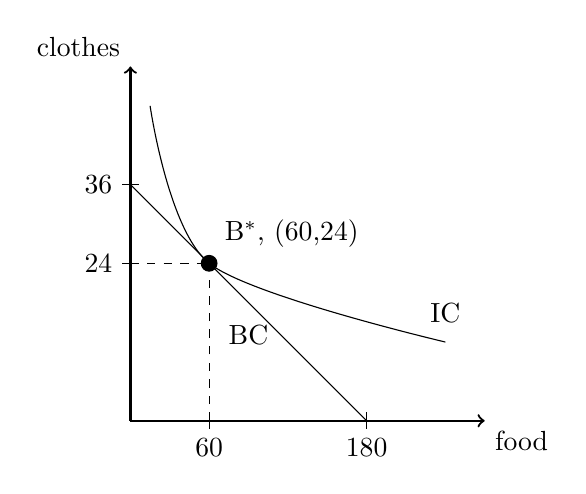
\begin{tikzpicture}[
            dot/.style={shape=circle, inner sep=2pt, draw, node contents=},
            circ/.style={shape=circle, inner sep=2pt, draw, fill}]
				\draw[thick,->] (0,0) -- (4.5,0) node[anchor=north west] {food};
				\draw[thick,->] (0,0) -- (0,4.5) node[anchor=south east] {clothes};
				\draw (3cm,3pt) -- (3cm,-3pt) node[anchor=north] {$180$}; 
				\draw (1cm,3pt) -- (1cm,-3pt) node[anchor=north] {$60$}; 

				\draw (3pt,3cm) -- (-3pt,3cm) node[anchor=east] {$36$};
				\draw (3pt,2cm) -- (-3pt,2cm) node[anchor=east] {$24$};
        
				\draw (0,3) -- node[circle,label=below:BC]{} (3,0);
				\draw plot [smooth] coordinates {(0.25,4) (1,2) (4,1)};
				\draw (4,1) node[label=above:IC]{};
				\draw (1,2) node[circ,label=above right:{B$^*$, (60,24)}]{};
				
				\draw[dashed] (1,0) -- (1,2);
				\draw[dashed] (0,2) -- (1,2);
 		\end{tikzpicture}
\end{center}

The curve labeled IC is the indifference curve tangent to the budget constraint BC. They meet at the optimal bundle B$^*$, which contains 60 food and 24 clothes.

\subsection*{g)}

If she purchases her optimal bundle, then she spends $60(5) = 300$, or $1/3$ of her total budget on food. Similarly, she will spend $24(25) = 600$, or $2/3$ of her total budget on clothing.

\subsection*{h)} 

We notice quickly that the share of her budget spent on a good is exactly the exponent assigned to the good in the utility function.

\subsection*{i)}

Instead of $900$, we can solve the system for an arbitrary budget $M$. In that case, we arrive at $5x + 10x = M$ from part \textbf{e.3} instead of $5x + 10x = 900$ (as this is the first step where $M$ does not vanish in the manipulated equations after taking the partial derivative), meaning that $x = \frac{M}{15}$ and that $y = \frac{2M}{75}$ for the optimal bundle. This yields shares of $\frac{M}{15}(5) = \frac{1}{3}M$ spent on food and $\frac{2M}{75}(25) = \frac{2}{3}M$ spent on clothing. This implies that the shares spent on the goods are fixed independently of budget.

\subsection*{Problem 4}

\subsection*{a)}
She needs to complete exercise such that for every 10 minutes of running (or mile ran) she swims 2 minutes. This means that if $x$ represents the miles run, then $10x + 2x = 60$, so she ought to run 5 miles and 500m (50 minutes running, 10 minutes swimming).

As an aside, Vera is very very fit. That's a lot of cardio!

\subsection*{b)}

\begin{center}
    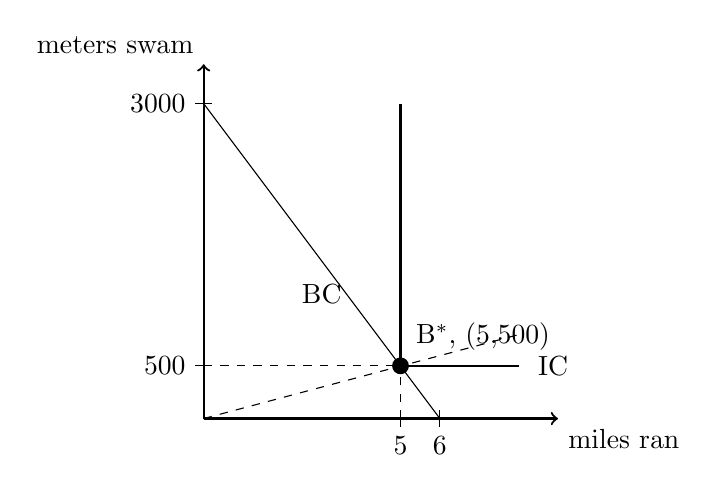
\begin{tikzpicture}[
            dot/.style={shape=circle, inner sep=2pt, draw, node contents=},
            circ/.style={shape=circle, inner sep=2pt, draw, fill}]
				\draw[thick,->] (0,0) -- (4.5,0) node[anchor=north west] {miles ran};
				\draw[thick,->] (0,0) -- (0,4.5) node[anchor=south east] {meters swam};
				\draw (3cm,3pt) -- (3cm,-3pt) node[anchor=north] {$6$}; 
				\draw (2.5cm,3pt) -- (2.5cm,-3pt) node[anchor=north] {$5$}; 

				\draw (3pt,4cm) -- (-3pt,4cm) node[anchor=east] {$3000$};
				\draw (3pt,0.67cm) -- (-3pt,0.67cm) node[anchor=east] {$500$};
        
				\draw (0,4) -- node[circle,label=below:BC]{} (3,0);
				\draw[thick] (2.5,4) -- (2.5,0.67) -- (4,0.67);
				\draw (4,.67) node[label=right:IC]{};
				\draw (2.5,0.67) node[circ,label=above right:{B$^*$, (5,500)}]{};
				
				\draw[dashed] (2.5,0) -- (2.5,0.67);
				\draw[dashed] (0,0.67) -- (2.5,0.67);
				\draw[dashed] (0,0) -- (4,1.066);
 		\end{tikzpicture}
\end{center}

The line marked BC is the budget constraint. The indifference curve, labeled IC, is shaped as an L as the two are perfect compliments. The optimal bundle is marked B$^*$, at 5 miles ran, 500m swam. The slanted dotted line marks the ratio at which Vera wants to split running and swimming.


\end{document}